\section{Results}\label{sec:results}

We report four experiments. E1 and E2 probe the geometry of the drama construct itself; E3 is the crux, asking whether reader disagreement is a threshold or a direction; E4 asks whether prompting a reader persona rotates the axis. The headline is a split: the construct is multi-dimensional (E1/E2), yet reader variation is overwhelmingly a threshold on a shared axis (E3/E4).

\para{E1: melodrama is a distinct excess direction, not more drama.} The presence of drama decodes essentially perfectly. A difference-in-means probe separates dramatic from neutral text at AUROC $1.000$ at every layer we test in \qwenbig\ (\tabref{tab:e1}). If melodrama were simply ``more drama,'' the dramatic$\to$melodramatic step would point along the same axis. It does not. {\bf Is melodrama just more drama?} At layer 16 the step is still nearly collinear with the drama axis ($\cos=0.999$, $56^\circ$), but it rotates steadily with depth, reaching $\cos=0.830$ and $83^\circ$ at the final layer---near orthogonal. \figref{fig:excess} makes the geometry explicit: dramatic and melodramatic items sit at the {\em same} value along the drama axis but pull apart along a second, near-orthogonal {\em excess} axis. \figref{fig:geometry}(a) shows the rotation is monotone in depth and replicates in \qwensmall\ (the step angle grows from $25^\circ$ to $85^\circ$). Melodrama is therefore not a higher threshold on the drama axis; it is a separate feature.

\begin{table}[t]\centering
\caption{Geometry of the drama construct in \qwenbig\ across depth. Drama decodes perfectly at every layer, yet the dramatic$\to$melodramatic step rotates toward orthogonality and the 8-subconcept participation ratio grows, so melodrama is a distinct direction, not a higher threshold on the drama axis.}
\label{tab:e1}
\begin{tabular}{@{}lcccc@{}}\toprule
Layer (rel.\ depth) & Drama AUROC & $\cos(\text{drama},\text{melo})$ & Angle of dramatic$\to$melo step & Subspace PR (of 8) \\\midrule
16 (0.57) & 1.000 & 0.999 & $56^\circ$ & 1.63 \\
21 (0.75) & 1.000 & 0.998 & $79^\circ$ & 2.18 \\
28 (1.0) & 1.000 & 0.830 & \textbf{$83^\circ$} & \textbf{5.64} \\
\bottomrule\end{tabular}\end{table}

\begin{figure}[t]\centering
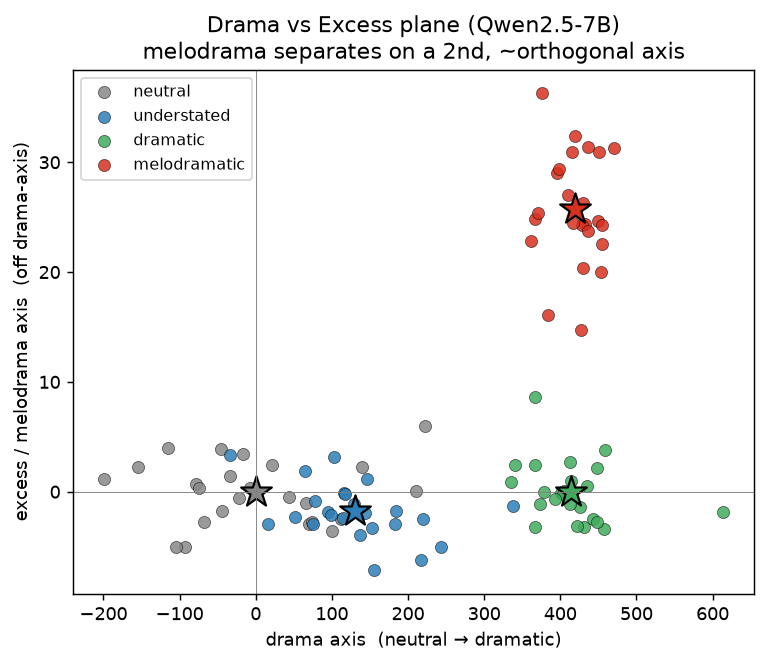
\includegraphics[width=0.55\linewidth]{figures/drama_excess_plane.png}
\caption{Dramatic (green) and melodramatic (red) items sit at the {\em same} drama-axis value but separate on a second, near-orthogonal excess axis (\qwenbig, final layer). Melodrama is off-axis, not further along it.}
\label{fig:excess}\end{figure}

\para{E2: the drama subspace is low-rank but multi-dimensional.} If drama were a single axis, the eight drama subconcepts (suspense, pathos/grief, spectacle, stakes, sincerity, excess/sentimentality, shock, restraint) would collapse onto one direction (participation ratio $\mathrm{PR}=1$); if they were unrelated, they would fill the space ($\mathrm{PR}\approx 8$). We find neither. The PR of the eight subconcept directions rises with depth to $\sim\!5.6$ in \qwenbig\ and $\sim\!5.9$ in \qwensmall\ (\tabref{tab:e1}, last column; \figref{fig:geometry}(b))---far below the random ceiling of $\sim\!8$ but well above $1$. Drama is a genuine {\em low-dimensional space} of features, not a single axis. The subconcept cosine structure is interpretable (\figref{fig:geometry}(c)): shock and suspense correlate, while pathos/grief and restraint anti-correlate, matching the intuition that built-up tension and emotional excess pull in opposite directions from quiet understatement.

\begin{figure}[t]\centering
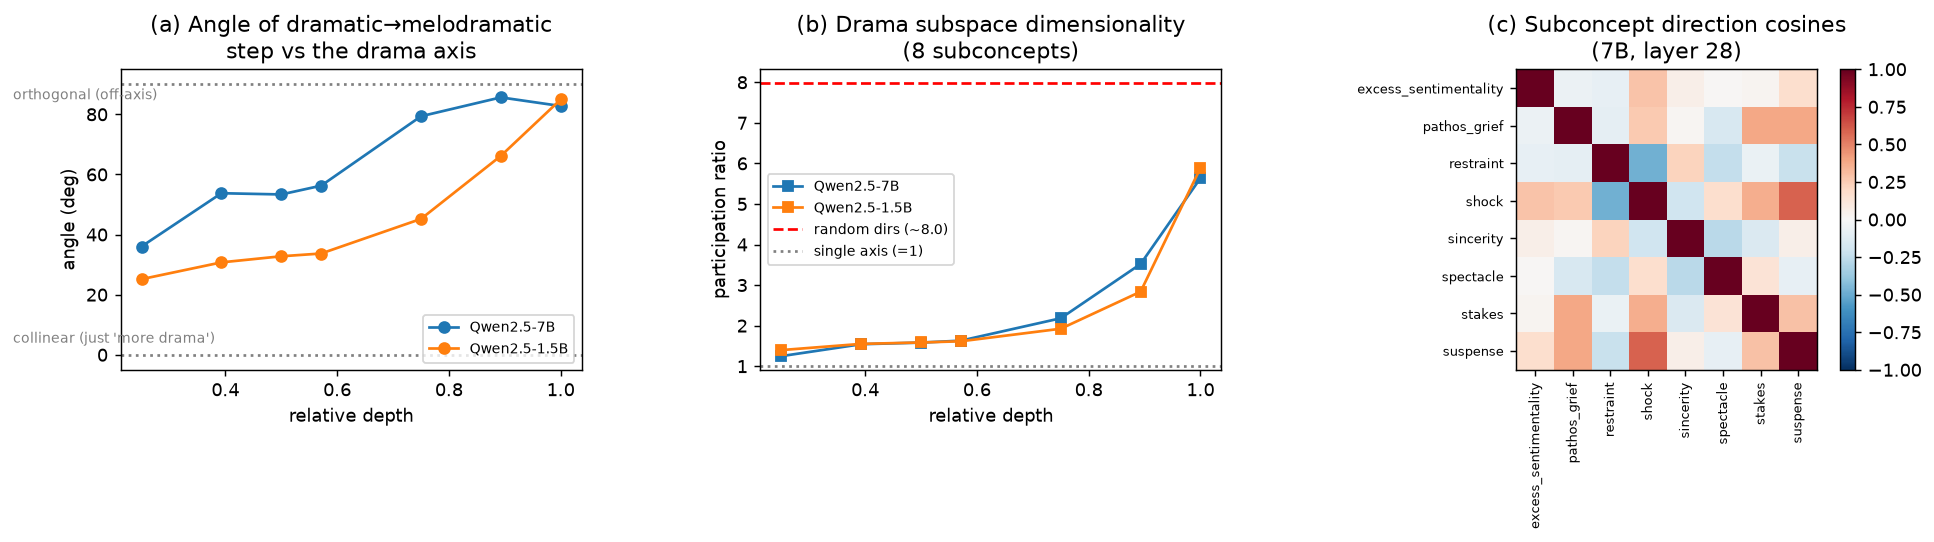
\includegraphics[width=\linewidth]{figures/e1_e2_geometry.png}
\caption{(a) The dramatic$\to$melodramatic step rotates from near-collinear to $\sim$80--86$^\circ$ with depth in both \qwenbig\ and \qwensmall; (b) the 8-subconcept participation ratio rises to $\sim$5.6--5.9, far below the random ceiling ($\sim$8) but well above a single axis (1); (c) interpretable subconcept cosine structure (shock$\leftrightarrow$suspense correlate; pathos/grief$\leftrightarrow$restraint anti-correlate).}
\label{fig:geometry}\end{figure}

\para{E3: reader variation is a threshold, not a direction.} Having shown the construct is multi-dimensional, we ask whether {\em readers} exploit those extra dimensions---whether disagreement is a reader-specific {\em direction} in the drama subspace (H2) or merely a per-reader {\em threshold} on a shared axis (H1). We fit a nested ladder of logistic models predicting each rater's binary drama label from text activations, evaluating on text-disjoint held-out items across $70$ \goemotions\ readers. \Mzero\ is a single shared axis; \Mone\ adds a per-reader threshold (intercept); \Mtwo\ adds a per-reader gain (slope); \Mthree\ lets each reader choose their own weight vector inside the drama subspace.

The transferred-corpus subspace (\dramacorpus, layer 21; \tabref{tab:e3transfer}, \figref{fig:e3}) tells the story cleanly. The decisive lift comes from the per-reader {\em threshold}: \Mzero\ at $0.510$ jumps to $0.619$ at \Mone. Everything after is flat---per-reader gain reaches only $0.622$ and a full reader-specific direction in the 9-D subspace reaches $0.623$. The added direction buys $\Delta(\Mthree-\Mtwo)=+0.0006$, exactly matching the shuffled-reader null of $+0.0006$ ($z=-0.5$): the gain is pure model capacity, present even when reader identities are randomized. The reader-weight matrix is low-rank ($\mathrm{PR}=3.25$ of $9$; \figref{fig:e3}, right), \ie\ what little reader-to-reader weight variation exists lives in a few shared dimensions, not in idiosyncratic per-reader directions.

\begin{table}[t]\centering
\caption{E3 nested held-out AUROC on a transferred \dramacorpus\ subspace (\qwenbig, layer 21, 70 readers, text-disjoint). The decisive lift is the per-reader threshold (\Mone); adding a reader-specific direction (\Mthree) matches the shuffled-reader null. Best simple model in \textbf{bold}.}
\label{tab:e3transfer}
\begin{tabular}{@{}lcc@{}}\toprule
Model & What it adds & Held-out AUROC \\\midrule
\Mzero shared single axis & --- & 0.510 \\
\Mone + per-reader threshold & reader intercept & \textbf{0.619} \\
\Mtwo + per-reader gain & reader slope (1-axis) & 0.622 \\
\Mthree + per-reader direction & weight vector in 9-D subspace & 0.623 \\
\bottomrule\end{tabular}\end{table}

The in-domain PCA subspace ($K{=}30$; \tabref{tab:e3indomain}, \figref{fig:e3b}) is the fairer test, since the drama directions are estimated from the same activation distribution the readers are evaluated on, and it reproduces the pattern at higher absolute AUROC. At layer 21, \Mzero\ scores $0.660$ and the per-reader threshold (\Mone) drives the jump to $0.700$; the shared $K$-dim subspace (\MtwoK) barely helps beyond one axis at $0.701$, and the reader-specific direction (\Mthree) reaches only $0.708$. The reader-direction effect $\Delta(\Mthree-\MtwoK)=+0.0076$ is {\em identical} to the shuffled-reader null of $+0.0076$ ($z=1.0$). Layer 28 repeats this ($0.641\to0.686\to0.687\to0.691$; $\Delta=+0.0046$ real vs.\ $+0.0046$ null, $z=-0.2$). Across both layers the decisive lift is $\Mzero\to\Mone$ ($+0.04$ to $+0.11$), the shared full subspace adds $\sim\!+0.001$ beyond one axis, and the reader-specific direction adds nothing beyond the null. \figref{fig:e3b}(b) shows the real reader-direction effect lying directly on top of the shuffled-reader null distribution. The cross-model replication in \qwensmall\ (layer 21) is identical in shape: $0.661\to0.702\to0.703\to0.711$, with $\Delta(\Mthree-\MtwoK)=+0.0084$ matching the null of $+0.0084$ ($z=0.28$). Reader disagreement is a threshold on a shared axis, not a reader-specific direction.

\begin{table}[t]\centering
\caption{E3 nested held-out AUROC on the in-domain PCA drama subspace ($K{=}30$), \qwenbig. The per-reader threshold (\Mone) drives the gain; the shared $K$-dim subspace barely helps beyond one axis, and the reader-specific direction (\Mthree) adds only the shuffled-reader null. Decisive threshold row in \textbf{bold}.}
\label{tab:e3indomain}
\begin{tabular}{@{}lcc@{}}\toprule
Model & Layer 21 & Layer 28 \\\midrule
\Mzero shared 1 axis & 0.660 & 0.641 \\
\Mone + reader threshold & \textbf{0.700} & \textbf{0.686} \\
\MtwoK shared $K$-dim + threshold & 0.701 & 0.687 \\
\Mthree reader-specific $K$-dim direction & 0.708 & 0.691 \\
$\Delta(\Mthree-\MtwoK)$ real vs.\ null & $+0.0076$ vs.\ $+0.0076$ ($z{=}1.0$) & $+0.0046$ vs.\ $+0.0046$ ($z{=}{-}0.2$) \\
\bottomrule\end{tabular}\end{table}

\begin{figure}[t]\centering
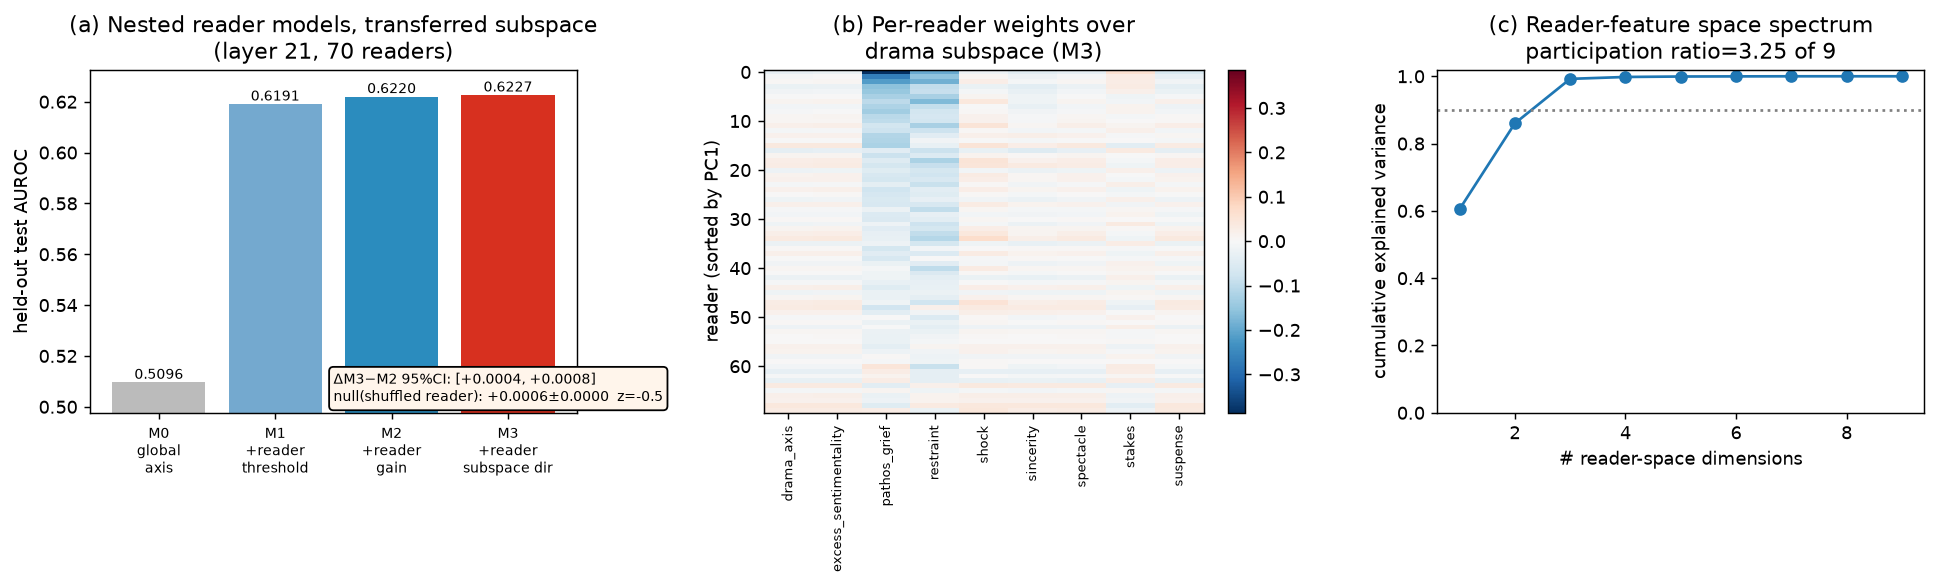
\includegraphics[width=\linewidth]{figures/e3_reader_models.png}
\caption{Transferred-subspace nested ladder (left), per-reader weights over the drama subspace (center), and the reader-feature spectrum (right, $\mathrm{PR}=3.25$ of 9). The per-reader threshold (\Mone) captures nearly all the gain; \Mthree\ adds only the null.}
\label{fig:e3}\end{figure}

\begin{figure}[t]\centering
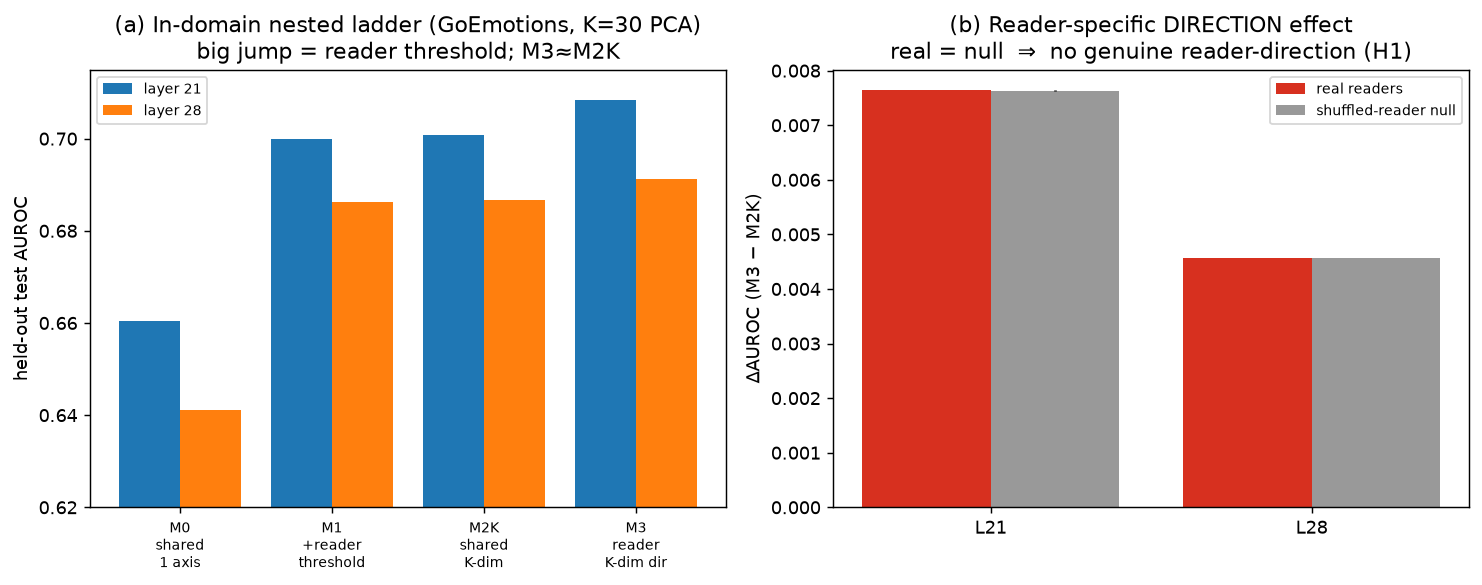
\includegraphics[width=\linewidth]{figures/e3b_indomain.png}
\caption{(a) In-domain nested ladder at layers 21/28---the big jump is the per-reader threshold (\Mzero$\to$\Mone) and \Mthree$\approx$\MtwoK; (b) the reader-specific direction effect $\Delta(\Mthree-\MtwoK)$ equals the shuffled-reader null, so it is pure model capacity, not genuine reader-direction structure.}
\label{fig:e3b}\end{figure}

\para{E4: prompting a persona does not rotate the drama axis.} Finally we re-derive the drama axis under six prompted reader personas (cynic, romantic, stoic, thrill-seeker, critic, neutral) using the chat template and a system persona. If different readers read along different directions, persona-conditioned axes should diverge. They do not: pairwise cosine between persona drama axes is $\geq 0.974$ (mean $0.99$), \ie\ all six personas recover essentially the same direction (\figref{fig:persona}(a)). The register ordering (neutral $<$ understated $<$ dramatic $<$ melodramatic) is unchanged across all personas (\figref{fig:persona}(b)). Prompting a reader shifts where the projection falls and where the threshold sits, but it does not rotate the axis---consistent with the E3 verdict that reader variation is a shared-axis threshold.

\begin{figure}[t]\centering
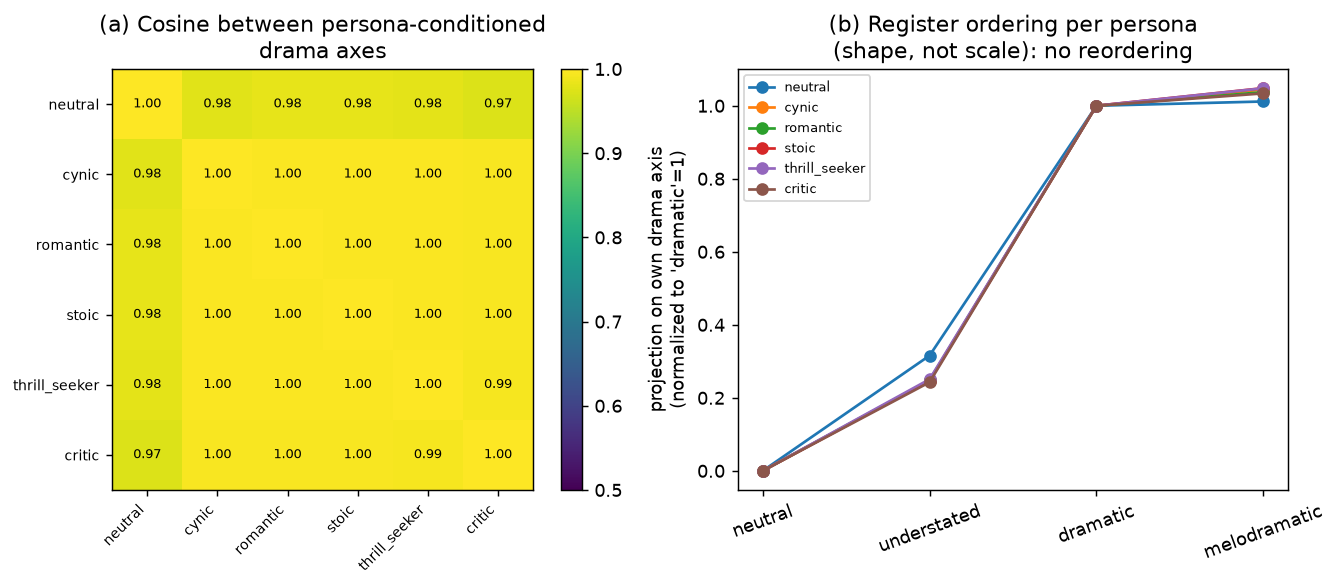
\includegraphics[width=\linewidth]{figures/e4_persona.png}
\caption{(a) Pairwise cosine between persona-conditioned drama axes is $\geq 0.974$ (mean $0.99$); (b) the register ordering is unchanged across personas. Prompting a reader shifts the projection/threshold, not the axis.}
\label{fig:persona}\end{figure}

Taken together, the construct is multi-dimensional---drama and melodrama occupy distinct, near-orthogonal directions (E1) within a low-rank but multi-dimensional subspace (E2)---yet readers share that geometry and differ almost entirely in {\em where} they place the threshold, not in {\em which} direction they read (E3, E4).
